% Created 2024-11-17 Sun 11:57
% Intended LaTeX compiler: pdflatex
\documentclass[letterpaper, 11pt]{article}
                                \usepackage{lmodern} % Ensures we have the right font
\usepackage[T1]{fontenc}
\usepackage[utf8]{inputenc}
\usepackage{graphicx}
\usepackage{amsmath, amsthm, amssymb}
\usepackage[table, xcdraw]{xcolor}
\definecolor{bblue}{HTML}{0645AD}
\usepackage[colorlinks]{hyperref}
\hypersetup{colorlinks, linkcolor=blue, urlcolor=bblue}
\usepackage{titling}
\setlength{\droptitle}{-6em}
\setlength{\parindent}{0pt}
\setlength{\parskip}{1em}
\usepackage[stretch=10]{microtype}
\usepackage{hyphenat}
\usepackage{ragged2e}
\usepackage{subfig} % Subfigures (not needed in Org I think)
\usepackage{hyperref} % Links
\usepackage{listings} % Code highlighting
\usepackage[top=1in, bottom=1.25in, left=1.55in, right=1.55in]{geometry}
\renewcommand{\baselinestretch}{1.15}
\usepackage[explicit]{titlesec}
\pretitle{\begin{center}\fontsize{20pt}{20pt}\selectfont}
\posttitle{\par\end{center}}
\preauthor{\begin{center}\vspace{-6bp}\fontsize{14pt}{14pt}\selectfont}
\postauthor{\par\end{center}\vspace{-25bp}}
\predate{\begin{center}\fontsize{12pt}{12pt}\selectfont}
\postdate{\par\end{center}\vspace{0em}}
\titlespacing\section{0pt}{5pt}{5pt} % left margin, space before section header, space after section header
\titlespacing\subsection{0pt}{5pt}{-2pt} % left margin, space before subsection header, space after subsection header
\titlespacing\subsubsection{0pt}{5pt}{-2pt} % left margin, space before subsection header, space after subsection header
\usepackage{enumitem}
\setlist{itemsep=-2pt} % or \setlist{noitemsep} to leave space around whole list
\author{Tatiana Dehoff, Finn Sparks, Jackson Mowry}
\date{Sun Nov 17 2024}
\title{Matrix Vector Multiplication\\\medskip
\large COSC 312 HW 8b: Extra Credit TM Project}
\hypersetup{
 pdfauthor={Tatiana Dehoff, Finn Sparks, Jackson Mowry},
 pdftitle={Matrix Vector Multiplication},
 pdfkeywords={},
 pdfsubject={},
 pdfcreator={Emacs 29.4 (Org mode 9.7.11)}, 
 pdflang={English}}
\begin{document}

\maketitle
\section{Project Description and Summary}
\label{sec:org35877a1}
We have built a matrix vector multiplication machine that accepts a matrix\textsubscript{n\texttimes{}n} and a vector\textsubscript{n\texttimes{}1}, producing the result of the calculation. Numbers are represented in unary notation with a single '1' for each digit. All numbers in the input must be \(\in\) \(\mathbb{W}\), that is the set of all whole numbers including 0. The machine supports any arbitrary sized matrix and vector, as long as the result of multiplication for the two operands is defined (i.e. we cannot multiply a 2\texttimes{}2 matrix by a 3\texttimes{}1 vector).\\

Our input space consists of \{\texttt{[}, \texttt{]}, \texttt{=}, \texttt{*}, \texttt{,}, \texttt{;}, \texttt{1}\} to represent the matrix/vector notation.\\
\subsection{Members}
\label{sec:org62a3e63}
\begin{itemize}
\item Tatiana Dehoff: (fill this in)\\
\item Finn Sparks: (fill this in)\\
\item Jackson Mowry: Implemented an initial rough draft of a matrix vector multiplicaiton machine. Wrote this report giving a summary and overview of our turing machine project.\\
\end{itemize}
\subsection{Matrix/Vector Notation}
\label{sec:org9ec4c6c}
Matricies and vectors are represented in a standard notation where \texttt{,} separates digits within the same row, and \texttt{;} separates rows in a matrix or vector. [1,2,3;4,5,6;7,8,9] is represented as\ldots{}\\
\[\begin{bmatrix}1&2&3\\4&5&6\\7&8&9\end{bmatrix}\]\\

\ldots{}and [1;2;3] is represented as\ldots{}\\
\[\begin{bmatrix}1\\2\\3\end{bmatrix}\]\\

To convert base\textsubscript{10} digits into unary digits we create a corresponding number of 1's in the notation. Once again converting [1,2;3,4] gives us\ldots{}\\
\[\begin{bmatrix}1&11\\111&1111\end{bmatrix}\]\\

\begin{figure}[htbp]
\centering
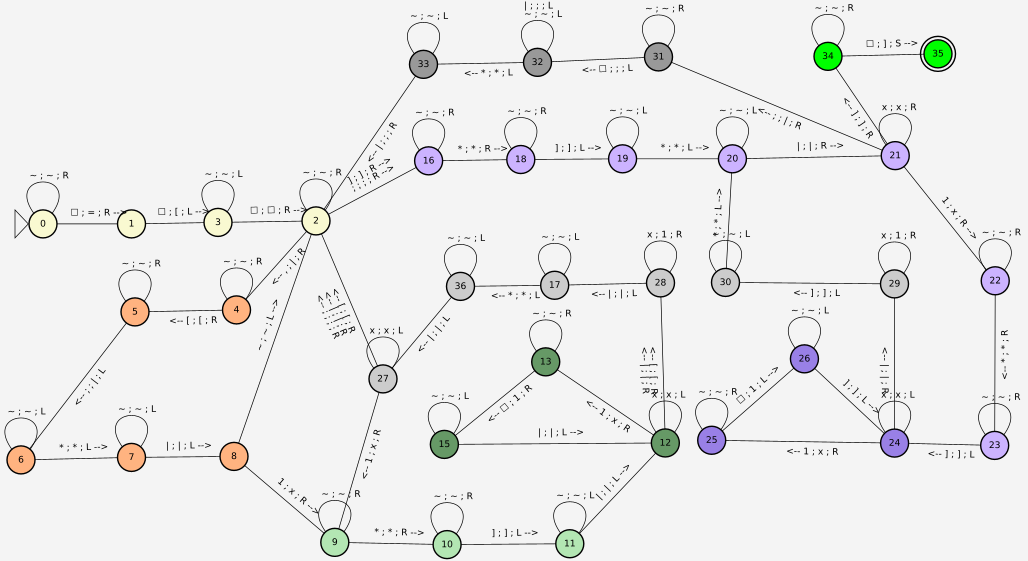
\includegraphics[width=5.5in]{2024-11-17_11-25.png}
\caption{Our final Turing Machine}
\end{figure}
\section{Turing Machine Functional Design}
\label{sec:org29868da}
\subsection{General Design}
\label{sec:org360a22c}
To begin our machine moves as far right as it can to write out \texttt{=} and \texttt{[} to prepare to write the resulting vector. After moving to the right it moves back to the start of input to begin multiplying each component in the matrix by its corresponding component in the vector. Once a single how to the matrix has been processed the machine will move into the result vector, write out a \texttt{;} to indicate the end of a digit, before finally resetting to the next row of the matrix. Once the machine reaches the end of the matrix (indicated by a \texttt{]}) it will traverse the far right and close off the result vector with a corresponding \texttt{]}.\\
\subsection{Pale Yellow}
\label{sec:orgb4eb239}
Pale yellow represents our start state, which is non-reentrant. The machine will move to the far right, write a \texttt{=} and \texttt{[}, then move back to the left of the tape input. This portion of the machine sets up the tape to begin writing the answer at the other end of the tape.\\
\subsection{Pale Orange}
\label{sec:org757ab1c}
Once the machine has set up the tape to begin writing the answer it starts to multiply the corresponding componenets of the matrix and vector together. The first step in this process is to identify which components we need to multiply. The machine accomplishes this by first marking off a comma in the matrix, then moving to the vector and finding the first comma that has not been marked off. Now that the component has been identified we can move on to unary multiplication by either consuming a 1 then moving to the light green stage, or if we're already looking at a \texttt{0} we just move to the next component of the matrix.\\
\subsection{Light Green}
\label{sec:orgd4e0b83}
Now that we are performing multiplication we can move to the right, looking for a \texttt{*} to identify the delimiter between the matrix and vector. Then we move to the end of the vector, turning around when we hit the end, then searching backwards for the \texttt{|} symbol. This allows us to always work on the last element that hasn't been crossed off, as opposed to starting from the begining which would be much more complicated to determine which element in the vector is being worked on. The machine will then break out of this loop once it finds the \texttt{|}, moving to the dark green portion of the machine to write out a \texttt{1} in the result vector.\\
\subsection{Dark Green}
\label{sec:org62a9a9e}
Now we can start writing out digits in the answer. Since we were just on top of a \texttt{|} symbol we know the digit to work on is sitting just to the left. We work on digits from right to left, meaning we may need to skip over some \texttt{x} characters in order to find the \texttt{1} that has not been crossed off. This is accomplished by looping on \texttt{x} and moving to the left. This loop is broken once we find a \texttt{1}, the machine then crosses this \texttt{1} off, replacing it with an \texttt{x}. Once a digit has been crossed off we need to write a \texttt{1} in the answer, which is accomplished by moving to the right until finding a blank, then writing a 1. The machine can then move back until finding a \texttt{|}, entering the beginning of the dark green loop.\\

The machine is only able to leave this dark green loop once it is done proccessing an entire component in the vector. This is indicated when we fine either another \texttt{|} or a \texttt{[} (indicating the start of the vector).\\
\subsection{Gray}
\label{sec:org630f6db}
Once the machine is done processing the appropriate component of the vector it will enter the gray set of states. The machine will now be at the left end of the digit, which means it can revert \texttt{x} to \texttt{1} while moving to the right, breaking out of this loop once it finds a \texttt{|} delimiter. This set of gray states then moves us to the left (out of the vector), and back into the matrix. This left moving loop is broken once we find a pipe, indicated that we are back at the component of the matrix we are working on. We then scan through all the \texttt{x} characters of this component to find the beginning. If we're done with this component of the matrix the machine will enter back into the pale orange loop described above.\\
\subsection{Light Purple}
\label{sec:org63d5673}
As we approach the end of a row in the vector our machine expects to see either a \texttt{;} or \texttt{]}. This indicates to the machine that it should now find the last component of the vector, as that is the corresponding element. It accomplishes this by moving to the right of the vector, and then coming back into the matrix looking for a pipe to indicate we are back the correct digit. After moving right off the pipe it should now be looking at either a \texttt{1} or an \texttt{x}, we consume any \texttt{x} characters until the machine is back on top of a \texttt{1}. This \texttt{1} is then marked off in the matrix, and the machine heads to the vector.\\
\subsubsection{Green}
\label{sec:org6fe4b9a}
As light purple is responsible for handling the last component in each row of the matrix, it must also be responsible for handling the accept state. As light purple is working on the last component in a row it is either looing for another 1 to multiply, or a \texttt{]}. Once it finds a \texttt{]} it knows the last element has been processed. The last step is to simply move to the far right, and place a \texttt{]} to close off the result vector and complete the calculation!\\
\subsection{Dark Purple}
\label{sec:orga596dab}
Working on the last component of the vector is treated differently, and we work on a digit from the right-hand side. Marking off each digit and copying it into the result vector one at a time. Once the first pass of the component has completed the machine heads to a short gray path.\\
\subsubsection{Gray}
\label{sec:orgecb21d4}
There is a short path here to revert \texttt{x} to \texttt{1} in the vector, before dumping us back into the matrix ready to process another digit. This then loops with the logic described above.\\
\subsection{Dark Gray}
\label{sec:orgadbacfe}
Once an entire row has been processed in the matrix the machine now needs to head to the right and write a \texttt{;} to mark the end of a row in the vector. This simply loops on any non-blank symbol while moving to the right. Once we find a blank we write a \texttt{;} and then perform the same loop consuming anything while moving to the left. The machine finally ends up back in the matrix ready to multiply another row by the vector. At this point the machine has been nearly fully explored, and it will continue looping until it has processed every digit, refer back to the light purple section for the accept state.\\
\subsection{Accept State}
\label{sec:org1a0f7ff}
Refer to the subsection \textbf{Green} above, as this is handled within the light purple path.\\
\section{How to Execute our Machine}
\label{sec:org11644ff}
The machine expects a matrix of dimensions n\texttimes{}n followed by \texttt{*} and then a vector of dimension n\texttimes{}1. All input values must be \(\in\) \(\mathbb{W}\), in unary notation.\\

\begin{center}
\begin{tabular}{r|r}
Base 10 & Unary\\
\hline
0 & \\
1 & 1\\
2 & 11\\
3 & 111\\
4 & 1111\\
5 & 11111\\
6 & 111111\\
7 & 1111111\\
8 & 11111111\\
9 & 111111111\\
10 & 1111111111\\
\end{tabular}
\end{center}

Each matrix/vector should be surround on either end with \texttt{[} and \texttt{]}, and the matrix should be separated from the vector with a \texttt{*} symbol. Componenets in the same row of the matrix are separated by \texttt{,} while rows of a matrix (and vector) are separated by \texttt{;}. Theoretically any dimension should be supported, however sizes larger than 4\texttimes{}4 or 5\texttimes{}5 tend to run very slowly.\\
\subsection{Accepted Input Values}
\label{sec:orgb6e3ec2}
\subsubsection{Example 1}
\label{sec:org2d8b9a9}
Valid input: \texttt{[1,11;111,1111]*[11;111]}\\
Expected output: \texttt{=[11111111;111111111111111111]}\\
or in base 10\ldots{}\\
\[\begin{bmatrix}1&2\\3&4\end{bmatrix}\begin{bmatrix}2\\3\end{bmatrix} = \begin{bmatrix}8\\18\end{bmatrix}\]\\
\subsubsection{Example 2}
\label{sec:org209a398}
Input with 0 present as a component in the matrix\\
Valid input: \texttt{[,1;11,111]*[11;111]}\\
Expected output: \texttt{=[111;1111111111111]}\\
or in base 10\ldots{}\\
\[\begin{bmatrix}0&1\\2&3\end{bmatrix}\begin{bmatrix}2\\3\end{bmatrix} = \begin{bmatrix}3\\13\end{bmatrix}\]\\
\subsubsection{Example 3}
\label{sec:orgf740b56}
Input with 0 present as a component in the vector\\
Valid input: \texttt{[1,1;11,111]*[;111]}\\
Expected output: \texttt{=[111;111111111]}\\
or in base 10\ldots{}\\
\[\begin{bmatrix}1&1\\2&3\end{bmatrix}\begin{bmatrix}0\\3\end{bmatrix} = \begin{bmatrix}3\\9\end{bmatrix}\]\\
\subsubsection{Example 4}
\label{sec:org46b8daa}
Input with a 0 matrix\\
Valid input: \texttt{[,;,]*[1111;11111]}\\
Expected output: \texttt{=[;]}\\
or in base 10\ldots{}\\
\[\begin{bmatrix}0&0\\0&0\end{bmatrix}\begin{bmatrix}4\\5\end{bmatrix} = \begin{bmatrix}0\\0\end{bmatrix}\]\\
\subsubsection{Example 5}
\label{sec:org4d9bea6}
Input with a 0 vector\\
Valid input: \texttt{[1,11;111,1111]*[;]}\\
Expected output: \texttt{=[;]}\\
or in base 10\ldots{}\\
\[\begin{bmatrix}1&2\\3&4\end{bmatrix}\begin{bmatrix}0\\0\end{bmatrix} = \begin{bmatrix}0\\0\end{bmatrix}\]\\
\subsubsection{Example 6}
\label{sec:org599b813}
Input with both 0 matrix and 0 vector\\
Valid input: \texttt{[,;,]*[;]}\\
Expected output: \texttt{=[;]}\\
or in base 10\ldots{}\\
\[\begin{bmatrix}0&0\\0&0\end{bmatrix}\begin{bmatrix}0\\0\end{bmatrix} = \begin{bmatrix}0\\0\end{bmatrix}\]\\
\subsubsection{Example 7}
\label{sec:org865ef19}
Input of dimension 3\\
Valid input: \texttt{[1,11,111;1,11,111;1,11,111]*[1;11;111]}\\
Expected output: \texttt{=[11111111111111;11111111111111;11111111111111]}\\
or in base 10\ldots{}\\
\[\begin{bmatrix}1&2&3\\1&2&3\\1&2&3\end{bmatrix}\begin{bmatrix}1\\2\\3\end{bmatrix} = \begin{bmatrix}14\\14\\14\end{bmatrix}\]\\
\end{document}
